\documentclass[aspectratio=169,12pt]{beamer}

%------------------------------------------------------------------
% Theme & colours
%------------------------------------------------------------------
\usetheme{Madrid}
\usecolortheme{default}
\setbeamertemplate{navigation symbols}{}
\setbeamertemplate{footline}[frame number]

%------------------------------------------------------------------
% Packages
%------------------------------------------------------------------
\usepackage{amsmath,amssymb,amsthm}
\usepackage{graphicx}
\usepackage{booktabs}
\usepackage{hyperref}
\usepackage{xcolor}
\usepackage{natbib}

%------------------------------------------------------------------
% Macros
%------------------------------------------------------------------
\newcommand{\E}{\mathbb{E}}
\newcommand{\R}{\mathbb{R}}
\newcommand{\dee}{\,\mathrm{d}}
\newcommand{\DKL}{D_{\mathrm{KL}}}

%------------------------------------------------------------------
% Title page
%------------------------------------------------------------------
\title[Heterogeneous Beliefs \& Markets]{Heterogeneous Beliefs and Financial Markets}
\subtitle{Based on Blume and Easley (2006) \\ QuantEcon Lecture 23}
\author{Thomas J.\ Sargent}
\institute{New York University}
\date{March 2026}

\begin{document}

%==================================================================
\begin{frame}
  \titlepage
\end{frame}

%==================================================================
\begin{frame}{Overview}

\textbf{Central question:} \emph{``If you're so smart, why aren't you rich?''} --- Blume and Easley (2006)

\bigskip
Blume and Easley study how \textbf{heterogeneous beliefs} about income-process probabilities influence:
\begin{itemize}
  \item consumption allocations
  \item prices of stocks, bonds, and insurance policies
  \item the long-run distribution of wealth among agents
\end{itemize}

\bigskip
\textbf{Historical backdrop:} Alchian (1950) and Friedman (1953) conjectured that competitive asset markets reward better-informed traders, transferring wealth to those with more realistic probability models.

\bigskip
This lecture provides a formal, tractable example with \textbf{complete markets}.

\end{frame}

%==================================================================
\begin{frame}{Roadmap}

\textbf{Two institutional arrangements\,---\,same outcome:}

\begin{enumerate}
  \item \textbf{Perfect socialism} --- a benevolent central planner dictates
        history-contingent consumption allocations.
  \item \textbf{Competitive markets} --- selfish price-taking agents trade
        contingent claims at equilibrium prices.
\end{enumerate}

\bigskip
The \textbf{two fundamental theorems of welfare economics} guarantee that these
arrangements produce \emph{identical allocations} once the planner's Pareto
weights are set appropriately.

\bigskip
\textbf{Key tool:} a \textbf{likelihood ratio process} links agents' relative
beliefs to their relative consumption shares across time and states.

\end{frame}

%==================================================================
\section{Likelihood Ratio Processes}

\begin{frame}{Review: Likelihood Ratio Processes}

\textbf{Setup.} A nonnegative random variable $W$ is drawn i.i.d.\ from
\emph{either} $f$ \emph{or} $g$.

\begin{itemize}
  \item Nature chooses the density \emph{once and for all} before time begins.
  \item Observers know both $f$ and $g$ but \emph{not} which one nature chose.
  \item We observe $\{w_t\}_{t=1}^{T}$ and want to infer nature's choice.
\end{itemize}

\bigskip
\textbf{Period-$t$ likelihood ratio:}
\[
  \ell(w_t)=\frac{f(w_t)}{g(w_t)}, \quad t\geq 1.
\]
Under density $g$, $\ell(w_t)$ is nonnegative with $\E_g[\ell(w_t)]=1$.

\bigskip
\textbf{Likelihood ratio process:}
\[
  L(w^t) = \prod_{i=1}^{t} \ell(w_i), \quad
  L(w^t) = \ell(w_t)\,L(w^{t-1}).
\]

\end{frame}

%==================================================================
\begin{frame}{Beta-Distribution Example}

\textbf{Concrete densities used throughout:}

\begin{center}
\renewcommand{\arraystretch}{1.3}
\begin{tabular}{lcc}
\toprule
Density & Distribution & Parameters \\
\midrule
$f$ & Beta & $(\alpha,\beta)=(1,\;1)$ \quad (uniform) \\
$g$ & Beta & $(\alpha,\beta)=(3,\;1.2)$ \\
\bottomrule
\end{tabular}
\end{center}

\bigskip
\begin{itemize}
  \item Both densities put positive probability on the same interval $(0,1)$.
  \item Simulation: draw $w_t \sim g$ and compute $L_t = \prod_{i=1}^t \ell(w_i)$.
  \item By the \textbf{law of large numbers}, $\log L_t \to -\DKL(g\|f)<0$
        almost surely when data come from $g$, so $L_t \to 0$.
\end{itemize}

\end{frame}

%==================================================================
\section{The Blume--Easley Model}

\begin{frame}{Blume and Easley's Setting}

\textbf{Aggregate endowment.}
At each date $t=0,1,2,\ldots$, a single nonstorable consumption good is
available in aggregate quantity \emph{one}:
\[
  y_t^1 + y_t^2 = 1.
\]

\begin{itemize}
  \item $s_t \in(0,1)$: i.i.d.\ draw from Beta$(\theta)$ --- \emph{nature's density} $\pi(s_t)$.
  \item Agent 1's endowment: $y_t^1 = s_t$.
  \item Agent 2's endowment: $y_t^2 = 1-s_t$.
\end{itemize}

\bigskip
\textbf{History.}
$s^t = (s_t, s_{t-1},\ldots,s_0)$, joint density
$\pi^t(s^t)=\pi(s_t)\cdots\pi(s_0)$.

\bigskip
\textbf{Feasibility:} $c_t^1(s^t)+c_t^2(s^t)=1$ for all $s^t$, all $t\geq 0$.

\end{frame}

%==================================================================
\begin{frame}{Nature and Agents' Beliefs}

\textbf{Nature} draws i.i.d.\ from its own density $\pi(s_t)$.

\bigskip
\textbf{Agents have heterogeneous beliefs:}
\begin{itemize}
  \item Agent $i$ believes nature draws from $\pi^i(s_t)$.
  \item Agent $i$ is \emph{mistaken} unless $\pi^i = \pi$.
  \item A \textbf{rational expectations model} would impose $\pi^i = \pi$ for all $i$.
\end{itemize}

\bigskip
\textbf{Our focus:}
\begin{itemize}
  \item Agent 1 believes marginal density $\pi^1(s_t) = f(s_t)$.
  \item Agent 2 believes marginal density $\pi^2(s_t) = g(s_t)$.
  \item Nature uses $\pi(s_t) = h(s_t)$, possibly a mixture of $f$ and $g$.
\end{itemize}

\bigskip
\textbf{Common discount factor:} $\delta \in (0,1)$.\\
\textbf{Common one-period utility:} $u(c) = \ln(c)$.

\end{frame}

%==================================================================
\begin{frame}{Intertemporal Utilities}

Agent $i$'s intertemporal expected utility:
\begin{equation}\label{eq:Vi}
  V^i = \sum_{t=0}^{\infty}\sum_{s^t} \delta^t\,u\!\left(c_t^i(s^t)\right)\pi_t^i(s^t).
\end{equation}

\begin{itemize}
  \item $\pi_t^i(s^t) = \pi^i(s_t)\cdots\pi^i(s_0)$ is agent $i$'s joint density over histories.
  \item Agent $i$ ranks consumption plans using \emph{their own subjective beliefs}.
\end{itemize}

\bigskip
\textbf{Social welfare criterion} (planner with Pareto weight $\lambda\in[0,1]$):
\[
  \mathcal{W} = \lambda\,V^1 + (1-\lambda)\,V^2.
\]

Setting $\lambda=0.5$ expresses \emph{egalitarian} social preferences.

\end{frame}

%==================================================================
\section{Social Planner's Problem}

\begin{frame}{Social Planner's Allocation Problem}

Maximise $\mathcal{W}=\lambda V^1+(1-\lambda)V^2$ subject to
$c_t^1(s^t)+c_t^2(s^t)=1$.

\bigskip
\textbf{First-order conditions} (dividing agent~1's FOC by agent~2's):
\[
  \frac{\pi_t^2(s^t)}{\pi_t^1(s^t)}\cdot
  \frac{1/c_t^2(s^t)}{1/c_t^1(s^t)}
  = \frac{\lambda}{1-\lambda}
  \quad\Longrightarrow\quad
  \frac{c_t^1(s^t)}{c_t^2(s^t)} = \frac{\lambda}{1-\lambda}\,l_t(s^t),
\]
where the \textbf{likelihood ratio}
\[
  l_t(s^t) = \frac{\pi_t^1(s^t)}{\pi_t^2(s^t)}
             = \prod_{i=0}^{t}\frac{f(s_i)}{g(s_i)}.
\]

\end{frame}

%==================================================================
\begin{frame}{The Planner's Allocation Rule}

Using feasibility $c_t^1+c_t^2=1$, the planner's rule is:
\begin{equation}\label{eq:c1star}
  \boxed{c_t^1(s^t) = \frac{\lambda\,l_t(s^t)}{1-\lambda+\lambda\,l_t(s^t)}.}
\end{equation}

\bigskip
\textbf{Continuation Pareto weights.} Define
\[
  \lambda_t(s^t) \;=\; \frac{\lambda\,l_t(s^t)}{1-\lambda+\lambda\,l_t(s^t)},
\]
so $c_t^1(s^t)=\lambda_t(s^t)$ and $c_t^2(s^t)=1-\lambda_t(s^t)$.

\bigskip
\begin{itemize}
  \item The continuation Pareto weight evolves endogenously with the
        likelihood ratio process.
  \item A \emph{smarter} agent (one whose beliefs better match nature's)
        sees $l_t\to\infty$ and therefore $\lambda_t\to 1$.
\end{itemize}

\end{frame}

%==================================================================
\section{If You're So Smart \ldots}

\begin{frame}{\textit{``If you're so smart, why aren't you rich?''}}

\textbf{Three limiting cases} for $l_\infty = \lim_{t\to\infty} l_t(s^\infty)$:

\bigskip
\begin{center}
\renewcommand{\arraystretch}{1.5}
\begin{tabular}{clcc}
\toprule
Case & Meaning & $l_\infty$ & $c_\infty^1$ \\
\midrule
1 & Both agents equally (un)smart & $1$ & $\lambda$ \\
2 & Agent 2 is smarter & $0$ & $0$ \\
3 & Agent 1 is smarter & $\infty$ & $1$ \\
\bottomrule
\end{tabular}
\end{center}

\bigskip
\begin{itemize}
  \item When beliefs are \emph{equally wrong}, consumption shares stay put at
        $(\lambda, 1-\lambda)$.
  \item When one agent is smarter, that agent eventually \emph{owns the entire
        endowment stream}.
  \item This is Alchian/Friedman, made precise.
\end{itemize}

\end{frame}

%==================================================================
\section{Competitive Equilibrium}

\begin{frame}{Competitive Equilibrium with Complete Markets}

\textbf{Setup.} At time $-1$, a complete set of \textbf{Arrow--Debreu} markets open.

\begin{itemize}
  \item Price $p_t(s^t)$: cost at $t=-1$ of one unit of consumption delivered at
        date $t$ after history $s^t$.
  \item Each agent takes prices as given and chooses $\{c_t^i(s^t)\}$ to
        maximise $V^i$ subject to:
\end{itemize}
\[
  \sum_{t\geq 0}\sum_{s^t} p_t(s^t)\,c_t^i(s^t)
  \;\leq\;
  \sum_{t\geq 0}\sum_{s^t} p_t(s^t)\,y_t^i(s^t).
\]

\textbf{FOC} for agent $i$ (attaching Lagrange multiplier $\mu^i$):
\[
  p_t(s^t) = \frac{\delta^t\,\pi_t^i(s^t)}{\mu^i\,c_t^i(s^t)}.
\]

\end{frame}

%==================================================================
\begin{frame}{Equilibrium Prices}

\textbf{Guess-and-verify.} Matching the competitive equilibrium with the
planning solution by setting $\mu^1=1-\lambda$ and $\mu^2=\lambda$:

\bigskip
\[
  \boxed{p_t(s^t) = \delta^t\,\lambda(1-\lambda)
    \Bigl[(1-\lambda)\,\pi_t^2(s^t)+\lambda\,\pi_t^1(s^t)\Bigr].}
\]

\bigskip
\textbf{Limiting cases:}

\begin{itemize}
  \item $l_\infty=0$ (agent~2 smarter): tails of prices reflect
        \emph{agent~2's} model, $p_t(s^t)\propto\delta^t\pi_t^2(s^t)$.
  \item $l_\infty=\infty$ (agent~1 smarter): tails of prices reflect
        \emph{agent~1's} model, $p_t(s^t)\propto\delta^t\pi_t^1(s^t)$.
  \item For small $t$: prices reflect a \emph{weighted mixture} of both models.
\end{itemize}

\bigskip
\textbf{Conclusion:} competitive equilibrium prices converge to reflect the
beliefs of the \emph{smarter} agent --- Alchian/Friedman confirmed.

\end{frame}

%==================================================================
\section{Simulations}

\begin{frame}{Simulation Design}

\textbf{Belief distributions:}
$f = \text{Beta}(1,1)$ (uniform), \quad $g = \text{Beta}(3,1.2)$.

\bigskip
\textbf{Three scenarios for nature's density $h$:}

\renewcommand{\arraystretch}{1.3}
\begin{center}
\begin{tabular}{ll}
\toprule
Scenario & Nature draws from \ldots \\
\midrule
Left   & $f$ (same as agent 1) \\
Middle & $g$ (same as agent 2) \\
Right  & $h = 0.5f + 0.5g$ (mixture) \\
\bottomrule
\end{tabular}
\end{center}

\bigskip
Parameters: $\lambda=0.5$, $T=100$ periods, $N=10{,}000$ simulated paths.

\bigskip
\textbf{Allocation rule} implemented:
\[
  c_t^1 = \frac{\lambda\,L_t}{1-\lambda+\lambda\,L_t},
  \quad L_t = \prod_{i=1}^{t}\frac{f(s_i)}{g(s_i)}.
\]

\end{frame}

%==================================================================
\begin{frame}{Simulation Results: Likelihood Ratios and Consumption Shares}

\begin{figure}
  \centering
  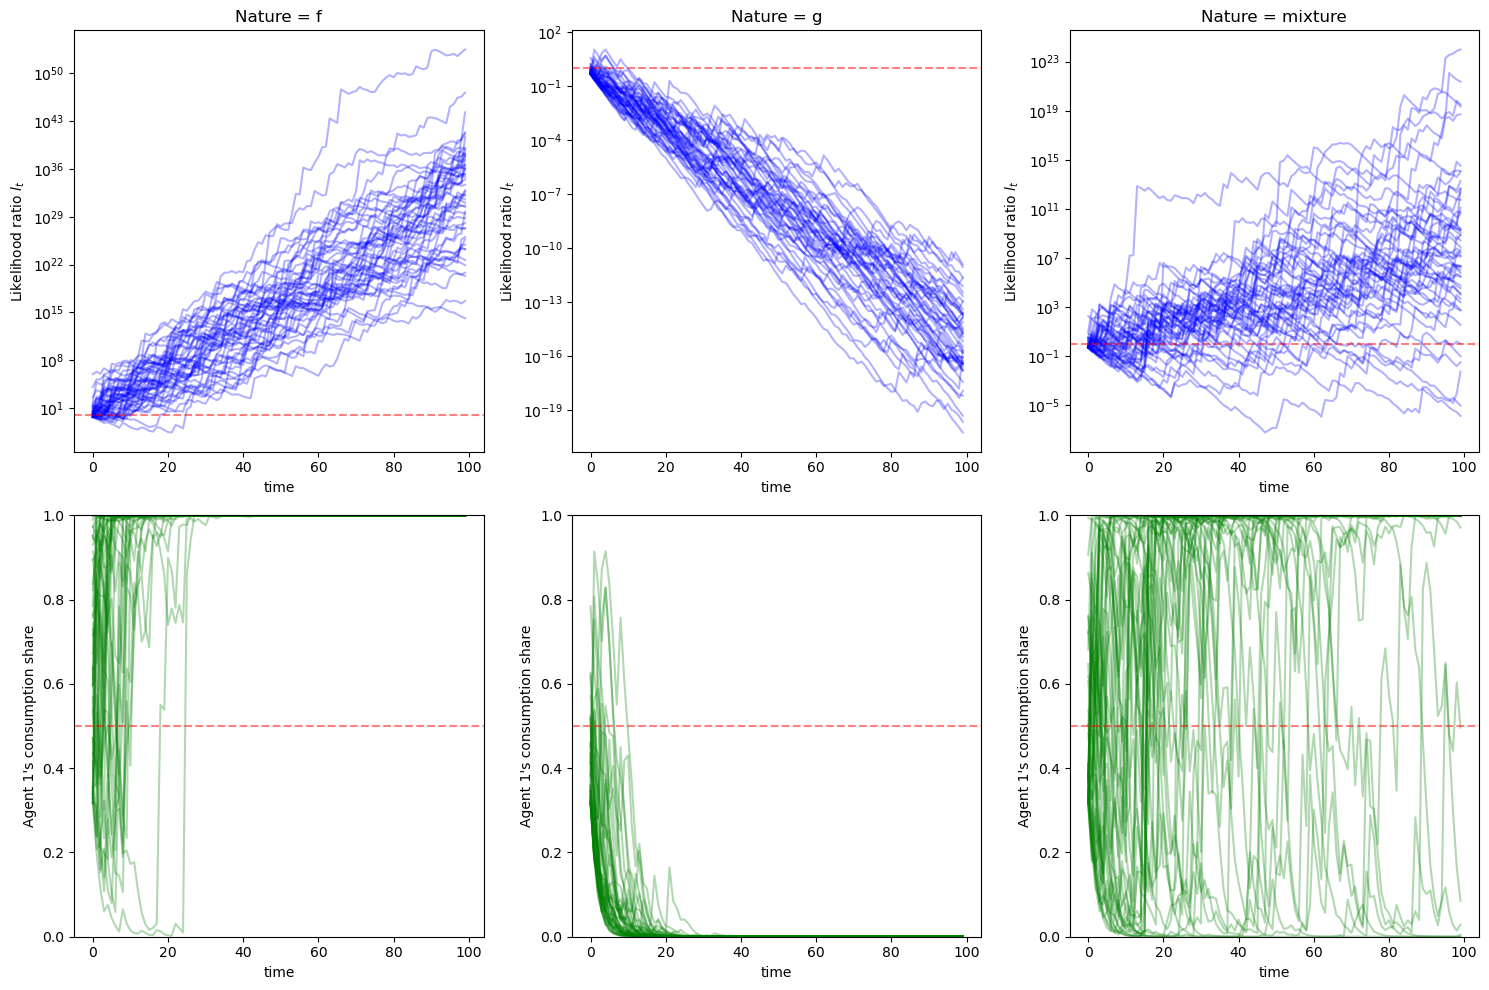
\includegraphics[width=0.92\linewidth,height=0.55\textheight,keepaspectratio]{lrp2_images/fig1_sim.png}
\end{figure}

\small
\textbf{Top row:} log-scale likelihood ratio paths for each scenario.
\textbf{Bottom row:} agent~1's consumption share paths ($\lambda=0.5$ dashed).\\
Left: nature$=f$ --- agent~1 quickly consumes everything.
Middle: nature$=g$ --- agent~1's share drifts to zero (more slowly).
Right: nature$=h$ --- mostly resembles the left panel since $\DKL(h\|g)>\DKL(h\|f)$.

\end{frame}

%==================================================================
\begin{frame}{KL Divergences: Key Numbers}

\textbf{Kullback--Leibler divergence} governs the rate of learning:
\[
  \DKL(p\|q) = \int p(w)\ln\!\frac{p(w)}{q(w)}\dee w \;\geq\; 0.
\]

\bigskip
\begin{center}
\renewcommand{\arraystretch}{1.4}
\begin{tabular}{lcc}
\toprule
Divergence & Value & Implication \\
\midrule
$\DKL(f,g)$ & $0.759$ & large surprise when one holds $g$ and nature is $f$ \\
$\DKL(g,f)$ & $0.344$ & moderate surprise in reverse case \\
$\DKL(h,f)$ & $0.073$ & $h$ is close to $f$ \\
$\DKL(h,g)$ & $0.281$ & $h$ is further from $g$ \\
\bottomrule
\end{tabular}
\end{center}

\bigskip
Since $\DKL(h,g)>\DKL(h,f)$, agent~1's beliefs ($f$) are \emph{closer} to
nature's mixture ($h$) than agent~2's beliefs ($g$).\\
$\Rightarrow$ Agent~1 ends up with final mean share $\approx 0.926$ when $h$ governs.

\end{frame}

%==================================================================
\begin{frame}{Close vs.\ Far Beliefs: Distributions}

\begin{figure}
  \centering
  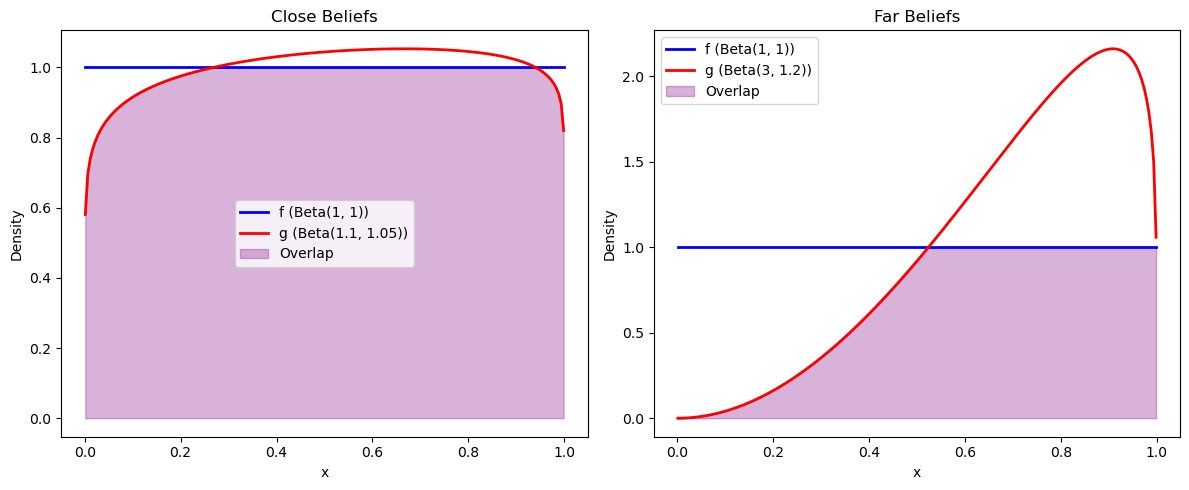
\includegraphics[width=0.80\linewidth,height=0.55\textheight,keepaspectratio]{lrp2_images/fig2_beliefs.png}
\end{figure}

\small
\textbf{Left:} ``Close'' beliefs: $f=\text{Beta}(1,1)$, $g=\text{Beta}(1.1,1.05)$ --- large overlap (purple).\\
\textbf{Right:} ``Far'' beliefs: $f=\text{Beta}(1,1)$, $g=\text{Beta}(3,1.2)$ --- small overlap.\\
Larger KL divergence $\Rightarrow$ faster convergence of consumption shares.

\end{frame}

%==================================================================
\begin{frame}{Close vs.\ Far: Consumption Share Dynamics}

\begin{figure}
  \centering
  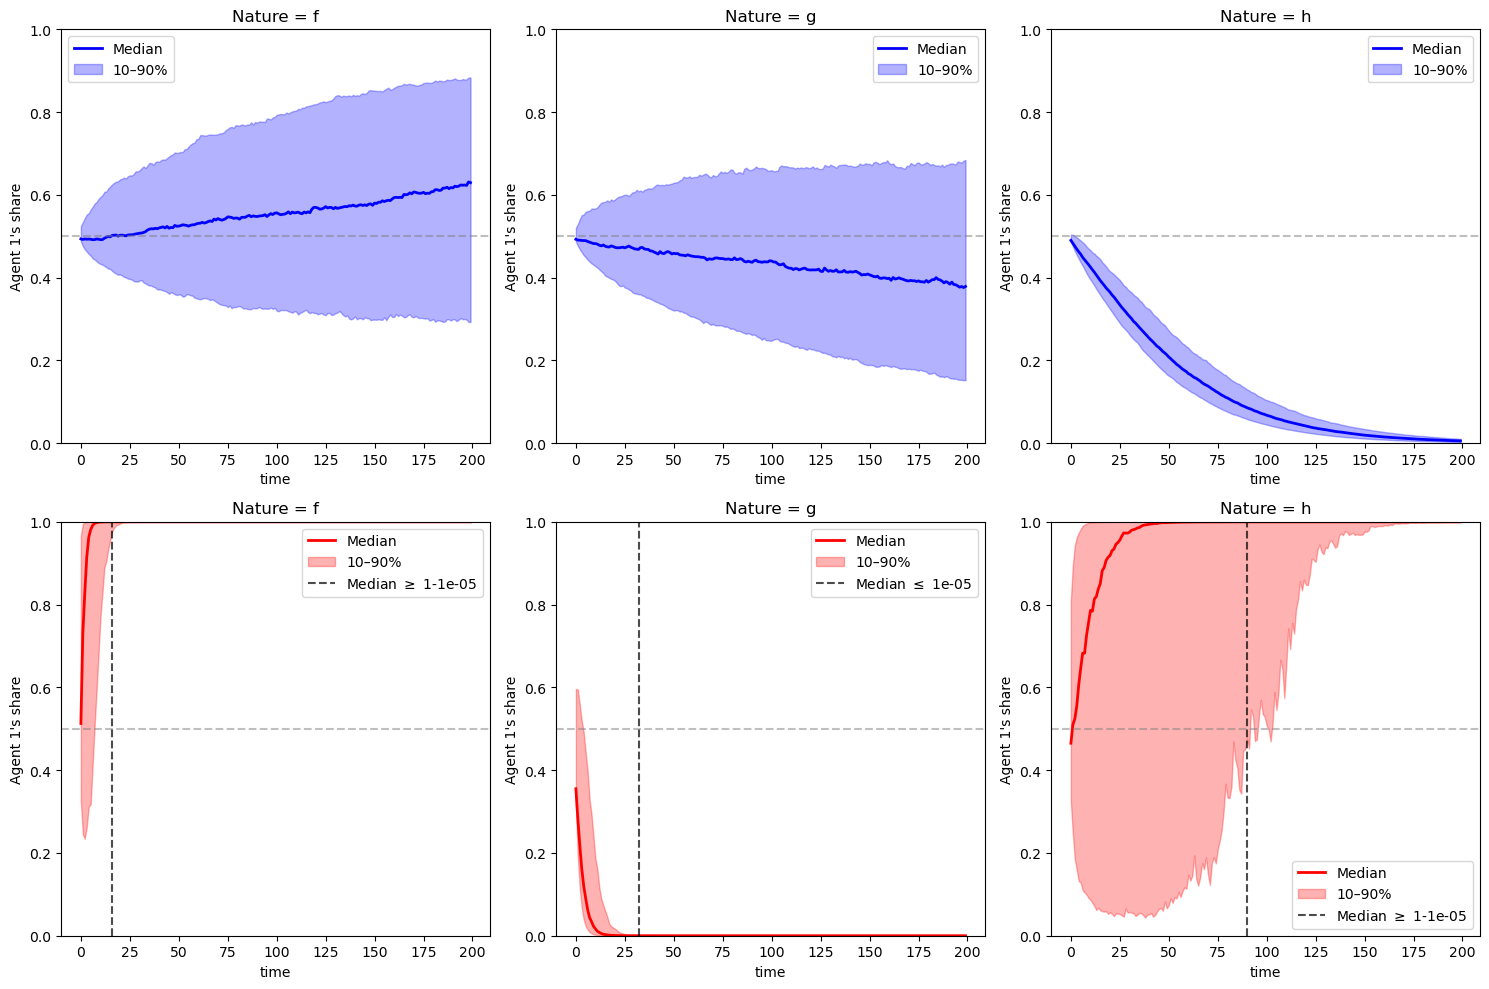
\includegraphics[width=0.92\linewidth,height=0.55\textheight,keepaspectratio]{lrp2_images/fig3_close_far.png}
\end{figure}

\small
\textbf{Top row} (close beliefs): convergence is \emph{slow} --- median paths linger near $\lambda=0.5$.\\
\textbf{Bottom row} (far beliefs): convergence is \emph{fast} --- dashed vertical lines show
the period at which the median share reaches near 0 or 1.\\
Within far beliefs, $\DKL(f,g)>\DKL(g,f)$ explains why convergence is faster when
nature chooses $f$ (left) than $g$ (middle).

\end{frame}

%==================================================================
\begin{frame}{KL Divergence Summary: Close vs.\ Far}

\begin{center}
\renewcommand{\arraystretch}{1.4}
\begin{tabular}{lcccc}
\toprule
Case & $\DKL(f,g)$ & $\DKL(g,f)$ & $\DKL(h,f)$ & $\DKL(h,g)$ \\
\midrule
Close & $0.003$ & $0.003$ & $0.073$ & $0.061$ \\
Far   & $0.759$ & $0.344$ & $0.073$ & $0.281$ \\
\bottomrule
\end{tabular}
\end{center}

\bigskip
\textbf{Observations:}
\begin{itemize}
  \item Close case: $\DKL(f,g)\approx\DKL(g,f)$, slow and symmetric convergence.
  \item Far case: $\DKL(f,g)\gg\DKL(g,f)$; faster convergence when nature$=f$
        than when nature$=g$.
  \item $\DKL(h,g)>\DKL(h,f)$ in both cases $\Rightarrow$ agent~1 is
        always closer to nature's mixture $h$.
\end{itemize}

\end{frame}

%==================================================================
\section{Summary}

\begin{frame}{Summary}

\begin{enumerate}
  \item \textbf{Likelihood ratio process} $l_t(s^t)=\pi_t^1(s^t)/\pi_t^2(s^t)$
        is the key state variable linking beliefs to allocations.

  \bigskip
  \item \textbf{Social planner's rule:} agent~1's consumption share equals
        the continuation Pareto weight
        $\lambda_t = \lambda\,l_t/(1-\lambda+\lambda\,l_t)$.

  \bigskip
  \item \textbf{Competitive equilibrium prices} are a Pareto-weighted average
        of agents' pricing kernels, converging to the smarter agent's kernel.

  \bigskip
  \item \textbf{Blume--Easley answer:} competitive markets do transfer wealth
        (and hence pricing power) to the better-informed agent, vindicating
        Alchian and Friedman --- but the \emph{rate} depends on KL divergences.

  \bigskip
  \item \textbf{KL divergence governs convergence speed:} the larger
        $\DKL(h\|g)$ relative to $\DKL(h\|f)$, the faster agent~1 accumulates
        consumption.
\end{enumerate}

\end{frame}

%==================================================================
\begin{frame}{Related Lectures and References}

\textbf{Related QuantEcon lectures:}
\begin{itemize}
  \item Lecture 22: \emph{Likelihood Ratio Processes} (foundations)
  \item Lecture 29: \emph{Likelihood Ratio Processes and Bayesian Learning}
  \item Lecture 88: \emph{Competitive Equilibria with Arrow Securities} (homogeneous beliefs)
  \item Lecture 89: \emph{Heterogeneous Beliefs and Bubbles} (Harrison--Kreps)
\end{itemize}

\bigskip
\textbf{Key references:}
\begin{itemize}
  \item Blume, L.\ and D.\ Easley (2006). ``If you're so smart, why aren't you
        rich?\ Belief selection in complete and incomplete markets.''
        \emph{Econometrica} 74(4), 929--966.
  \item Alchian, A.\ (1950). ``Uncertainty, evolution, and economic theory.''
        \emph{Journal of Political Economy} 58(3), 211--221.
  \item Friedman, M.\ (1953). \emph{Essays in Positive Economics}.
        University of Chicago Press.
\end{itemize}

\end{frame}

%==================================================================
\begin{frame}{Exercises (Selected)}

\textbf{Exercise 1.} Starting from the first-order condition
$p_t(s^t) = \delta^t\pi_t^i(s^t)/(\mu^i c_t^i(s^t))$, derive
\[
  p_t(s^t) = \delta^t\lambda(1-\lambda)\bigl[(1-\lambda)\pi_t^2(s^t)+\lambda\pi_t^1(s^t)\bigr].
\]

\bigskip
\textbf{Exercise 2.} Bayesian agents: each agent updates a prior over $f$ vs.\ $g$.
\begin{itemize}
  \item Set $f\sim\text{Beta}(1.5,1)$ and $g\sim\text{Beta}(1,1.5)$.
  \item Study consumption share dynamics and learning speed for different
        initial priors $\pi_0^1\neq\pi_0^2$.
\end{itemize}

\bigskip
\textbf{Exercise 3.} Same as Exercise 2 but with more separated distributions:
$f\sim\text{Beta}(2,5)$, $g\sim\text{Beta}(5,2)$.
Compare convergence speeds with the close-beliefs case.

\bigskip
\textbf{Exercises 4--5.} Two agents, three possible models ($f$, $g$, $h$):
study how extreme priors affect posterior evolution and consumption allocations.

\end{frame}

%==================================================================
\end{document}
